% latex uft-8
\documentclass[uplatex,a4paper,11pt,oneside,openany]{jsbook}
%
\usepackage[dvipdfmx]{graphicx}
\usepackage[dvipdfmx]{color}
\usepackage{amsmath,amssymb}
\usepackage{enumerate}
\usepackage{bm}
\usepackage{graphicx}
\usepackage{ascmac}
\usepackage{setspace}
\usepackage{here}
\usepackage{url}
\usepackage{comment}
\usepackage{listings,jlisting} %日本語のコメントアウトをする場合jlistingが必要
%ここからソースコードの表示に関する設定
\lstset{
%プログラム言語(複数の言語に対応,C,C++も可)
language = C,
%背景色と透過度
backgroundcolor = {\color[gray]{.95}},
%枠外に行った時の自動改行
breaklines = true,
%自動改行後のインデント量(デフォルトでは20[pt])
breakindent = 10pt,
%標準の書体
%basicstyle = \ttfamily\scriptsize,
basicstyle = \fontsize{8}{10}\selectfont\ttfamily,
%コメントの書体
commentstyle = {\itshape \color[cmyk]{1,0.4,1,0}},
%関数名等の色の設定
classoffset = 0,
%キーワード(int, ifなど)の書体
keywordstyle = {\bfseries \color[cmyk]{0,1,0,0}},
%表示する文字の書体
stringstyle = {\ttfamily \color[rgb]{0,0,1}},
%枠 "t"は上に線を記載,"T"は上に二重線を記載
%他オプション:leftline,topline,bottomline,lines,single,shadowbox
frame = TBrl,
%frameまでの間隔(行番号とプログラムの間)
framesep = 5pt,
%行番号の位置
numbers = left,
%行番号の間隔
stepnumber = 1,
%行番号の書体
numberstyle = \tiny,
%タブの大きさ
tabsize = 4,
%キャプションの場所("tb"ならば上下両方に記載)
captionpos = t
}
%ここまでソースコードの表示に関する設定
\makeatletter
\def\ps@plainfoot{%
\let\@mkboth\@gobbletwo
\let\@oddhead\@empty
\def\@oddfoot{\normalfont\hfil-- \thepage\ --\hfil}%
\let\@evenhead\@empty
\let\@evenfoot\@oddfoot
}
\let\ps@plain\ps@plainfoot
\renewcommand{\chapter}{%
\if@openright\cleardoublepage\else\clearpage\fi
\global\@topnum\z@
\secdef\@chapter\@schapter
}
\makeatother
%
\newcommand{\maru}[1]{{\ooalign{%
\hfil\hbox{$\bigcirc$}\hfil\crcr%
\hfil\hbox{#1}\hfil
}
}}
%
\setlength{\textwidth}{\fullwidth}
\setlength{\textheight}{40\baselineskip}
\addtolength{\textheight}{\topskip}
\setlength{\voffset}{-0.55in}
%
\begin{document}
% START DOCUMENT
%
% COVER
\begin{center}
\huge \_ \par
\vspace{25mm}
\LARGE 2022年度 ソフトウェア技術 \par
\vspace{15mm}
\huge C言語[演習] \par
\vspace{100mm}
\Large \today \par
\vspace{15mm}
\Large S.Matoike \par
\vspace{10mm}
\Large \par
\vspace{10mm}
\end{center}
\thispagestyle{empty}
\clearpage
\addtocounter{page}{-1}
\newpage
\setcounter{tocdepth}{3}
%
\tableofcontents
%
%%%%\chapter{はじめに}
%
\chapter{三目並べ(Tic Tac Toe)}

\section{ゲームの概要}

プログラムを実行すると、盤面が表示され、
×の石を置く場所を指定するよう促されます。

画面上に示された番号を入力すると、
その番号のスロットに×の石が置かれた盤面が表示され、
次の手番の○に、石を置く場所を指定するように促されます。

手番を交互に変えながらゲームは進み、縦、横、斜めの何れかに、
先に一列に自分の石を並べた方が勝ちとなります。

既に石の置かれているスロット番号を指定することはできません。
また、スロット番号として 0 〜 8 以外の数値を指定することもできません。

\begin{spacing}{0.74}
  \begin{verbatim}
    スタート! [Tic Tac Toe]
    /---|---|---\
    | 0 | 1 | 2 |
    |---|---|---|
    | 3 | 4 | 5 |
    |---|---|---|
    | 6 | 7 | 8 |
    \---|---|---/
    'X' さんのturnです
    石を置く場所 0 〜 8 を指定して下さい : 4
    /---|---|---\
    | 0 | 1 | 2 |
    |---|---|---|
    | 3 | X | 5 |
    |---|---|---|
    | 6 | 7 | 8 |
    \---|---|---/
    'O' さんのturnです
    石を置く場所 0 〜 8 を指定して下さい : 2
    /---|---|---\
    | 0 | 1 | O |
    |---|---|---|
    | 3 | X | 5 |
    |---|---|---|
    | 6 | 7 | 8 |
    \---|---|---/
    'X' さんのturnです
    石を置く場所 0 〜 8 を指定して下さい :
  \end{verbatim}
\end{spacing}

\section{主処理(main)}

\begin{lstlisting}[]
int main(int argc, char *argv[]){
    /* 先手後手を決定 */
    int turn = BATSU,  winner, num;
    if (1 < argc){
        if (!strcmp(argv[1], "-r"))
            turn = MARU;
    }
    printf("スタート! [Tic Tac Toe]\n");
    do{
        printBoard();            /* ①盤面の表示 */
        num = slotNum(turn); /* ②手を入力 */
        board[num] = turn;       /* ③手を盤面に配置 */
        turn = switchTurn(turn); /* ④手番の交代 */
        winner = checkWinner();  /* ⑤勝敗の判定 */
    } while (winner == NEXT);
    /* 対戦結果の表示 */
    printBoard();
    result(winner);
    return 0;
}
\end{lstlisting}

\section{盤面の表示(printBoard)}

\begin{lstlisting}
void printBoard() {
    char bd[9];
    int i;
    for (i = 0; i < 9; i++) {
        if (board[i] == MARU) bd[i] = 'O';
        else if (board[i] == BATSU) bd[i] = 'X';
        else bd[i] = '0' + i;
    }
    printf("\n/---|---|---\\\n");
    printf("| %c | %c | %c |\n", bd[0], bd[1], bd[2]);
    printf("|---|---|---|\n");
    printf("| %c | %c | %c |\n", bd[3], bd[4], bd[5]);
    printf("|---|---|---|\n");
    printf("| %c | %c | %c |\n", bd[6], bd[7], bd[8]);
    printf("\\---|---|---/\n");
}
\end{lstlisting}

\section{手番の交代(switchTurn)}

\begin{lstlisting}
int switchTurn(int turn) {
    if (turn== BATSU)return MARU;
    return BATSU;
}
\end{lstlisting}

\section{入力(slotNum)}

\begin{lstlisting}
int slotNum(int turn) {
    int num;
    char *fig = "";
    if (turn==MARU) fig = "'O'";
    else if (turn==BATSU) fig = "'X'";
    do {
        printf("\n %s さんのturnです\n石を置く場所 0 〜 8 を指定して下さい:", fig);
        //while (getchar() != '\n');  /* 標準入力バッファのクリア */
        scanf("%d", &num);
        if (!(0 <= num && num < 9)) {
            printf("再指定:0 〜 8 を指定して下さい");
            continue;
        }
        if (board[num] != num) {
            printf("再指定:そこには既に石が置かれています\n");
            continue;
        }
        break;
    } while (1);
    return num;
}
\end{lstlisting}

\section{判定(checkWinner)}

\begin{lstlisting}
int lineSum(int n1, int n2, int n3) {
    return board[n1] + board[n2] + board[n3];
}
int checkWinner() {
    int i, line = 0;
    for (i = 0; i < 8; i++) {
        switch (i) {
        case 0: line = lineSum(0, 1, 2); break;
        case 1: line = lineSum(3, 4, 5); break;
        case 2: line = lineSum(6, 7, 8); break;
        case 3: line = lineSum(0, 3, 6); break;
        case 4: line = lineSum(1, 4, 7); break;
        case 5: line = lineSum(2, 5, 8); break;
        case 6: line = lineSum(0, 4, 8); break;
        case 7: line = lineSum(2, 4, 6); break;
        }
        if (line == 3 * MARU) return MARU;
        else if (line == 3 * BATSU) return BATSU;
    }
    for (i = 0; i < 9; i++){
        if (0 <= board[i] && board[i] < 9) return NEXT;
    }
    return DRAW;
}
\end{lstlisting}

\newpage

\section{結果表示(result)}

\begin{lstlisting}
void result(int winner) {
    printf("\n");
    switch (winner) {
    case DRAW: printf("引き分け\t"); break;
    case MARU: printf("'O' の勝ち\t"); break;
    case BATSU: printf("'X' の勝ち\t"); break;
    }
    printf("またね!\n");
}
\end{lstlisting}

\section{各種宣言など}

これは冒頭に記述する

\begin{lstlisting}
#include <stdio.h>
#include <string.h>
  
// function prototypes
/*
int lineSum(int, int, int);
int switchTurn(int);
void printBoard();
int slotNum(int);
int checkWinner();
void result(int);
*/
  
static int board[] = {0, 1, 2, 3, 4, 5, 6, 7, 8};
#define MARU 10
#define BATSU -10
#define DRAW 100
#define NEXT 200
\end{lstlisting}

%\section{プログラムの全体}

%\lstinputlisting[caption=Tic Tac Toe(三目並べ),label=tictactoe]{tictactoe.c}

\chapter{スライド・パズル(15Puzzle)}

\section{ゲームの概要}

$4 \times 4$に区切った盤面上の各タイルに、$0〜15$の番号が割り振られている。
0 が割り振られたタイルは空欄になっていて、他のタイルはその空欄にスライドさせて
移動することができる。
最初は不規則に並べられている盤面ですが、空欄の上下、あるいは空欄の左右のタイルを
選んでは、空欄の方向にスライドさせる事によって、最終的に1から15まで規則正しく
並んだ盤面状態を目指すゲームである。

\begin{spacing}{0.74}
  \begin{verbatim}
% ./slidetile

[11][ 3][ 6][10]
[ 9][ 1][ 8][14]
[ 2][ 4][ 7][12]
[13][15][  ][ 5]

Select number:6

[11][ 3][  ][10]
[ 9][ 1][ 6][14]
[ 2][ 4][ 8][12]
[13][15][ 7][ 5]

Select number:11

[  ][11][ 3][10]
[ 9][ 1][ 6][14]
[ 2][ 4][ 8][12]
[13][15][ 7][ 5]

Select number:11

[11][  ][ 3][10]
[ 9][ 1][ 6][14]
[ 2][ 4][ 8][12]
[13][15][ 7][ 5]

Select number:
  \end{verbatim}
\end{spacing}

\section{主処理(main)}

\begin{lstlisting}
int main(void) {
    int sel;
    init();
    do {
        disp();
        do {
            printf("\nSelect number:");
            scanf("%d", &sel);
        } while( sel>ROW*COLUMN );
        moveTile(sel);
    } while( check() );

    return 0;
}
\end{lstlisting}

\section{盤面の初期化(init)}

乱数を使ってタイルをシャフルするので、
時刻を乱数の種に指定することによって、
プログラムを起動する度に、異なるタイル配置になる様にしている

\begin{lstlisting}
void init(){
    int i, j, n;
    srand((unsigned)time(NULL));
    for (i = 0; i < ROW; i++){
        for (j = 0; j < COLUMN; j++){
            n = i * COLUMN + j;
            tiles[n].num = n;
            tiles[n].row = i;
            tiles[n].clm = j;
        }
    }
    shuffle(1000);
}
\end{lstlisting}

\section{シャッフル(shuffle)}

乱数を使って、タイルを不規則に選択し移動させている

\begin{lstlisting}
void shuffle(int n){
    int sel, min = 0, max = ROW*COLUMN;
    do{
        sel = (rand() % (max - min + 1)) + min;
        moveTile(sel);
        n--;
    } while (0 < n);
}
\end{lstlisting}

\newpage

\section{盤面の表示(disp)}

\begin{lstlisting}
void disp(){
    int i, j, n;
    printf("\n");
    for (i = 0; i < ROW; i++){
        for (j = 0; j < COLUMN; j++){
            n = i * COLUMN + j;
            if (tiles[n].num == 0){
                printf("[  ]");
            } else {
                printf("[%2d]", tiles[i * COLUMN + j].num);
            }
        }
        printf("\n");
    }
}
\end{lstlisting}

\section{タイルのスライド(moveTile)}

\begin{lstlisting}
int findTileNum(int num){
    int i;
    for (i = 0; i < ROW * COLUMN; i++){
        if (tiles[i].num == num){
            return i;
        }
    }
    return -1;
}
void swapTile(int n1, int n2){
    int tmp = tiles[n1].num; 
    tiles[n1].num = tiles[n2].num;
    tiles[n2].num = tmp;
}
void swapTileR(int c, int r1, int r2){
    int n1 = r1 * COLUMN + c;
    int n2 = r2 * COLUMN + c;
    swapTile(n1, n2);
}
void swapTileC(int r, int c1, int c2){
    int n1 = r * COLUMN + c1;
    int n2 = r * COLUMN + c2;
    swapTile(n1, n2);
}
void moveTile(int sel){
    int j;
    int s = findTileNum(sel);
    int sr = tiles[s].row;
    int sc = tiles[s].clm;
    int z = findTileNum(0);
    int zr = tiles[z].row;
    int zc = tiles[z].clm;
    if (sr == zr){
        if (sc < zc){
            for (j = zc; j > sc; j--){
                if (0 <= j - 1){
                    swapTileC(sr, j, j - 1);
                }
            }
        } else if (zc < sc) {
            for (j = zc; j < sc; j++){
                if (j + 1 < COLUMN){
                    swapTileC(sr, j, j + 1);
                }
            }
        }
    }
    if (sc == zc){
        if (sr < zr){
            for (j = zr; j > sr; j--){
                if (0 <= j - 1){
                    swapTileR(sc, j, j - 1);
                }
            }
        } else if (zr < sr){
            for (j = zr; j < sr; j++){
                if (j + 1 < ROW){
                    swapTileR(sc, j, j + 1);
                }
            }
        }
    }
}
\end{lstlisting}

\section{完成チェック(check)}

\begin{lstlisting}
enum BOOLEAN check(){
    int i, j, n;
    for (i = 0; i < ROW; i++){
        for (j = 0; j < COLUMN; j++){
            n = i * COLUMN + j;
            if (tiles[n].num != n){
                return true;
            }
        }
    }
    return false;
}
\end{lstlisting}

\section{各種宣言など}

これは冒頭に記述する

\begin{lstlisting}
#include <stdio.h>
#include <stdlib.h>
#include <time.h>
  
// 定数
#define ROW 4
#define COLUMN 4
// 構造体
struct Tile{
      int num;
      int row;
      int clm;
};
enum BOOLEAN{
    false, /* false = 0, true = 1 */
    true
};
// function prototypes
/*
int findTileNum(int);
void swapTile(int,int);
void swapTileR(int,int,int);
void swapTileC(int,int,int);
void moveTile(int);
void shuffle(int);
enum BOOLEAN check();
void disp();
void init();
*/
  
static struct Tile tiles[16];   /* 16 = ROW * COLUMN */
\end{lstlisting}

%\section{プログラムの全体}

%\lstinputlisting[caption=スライド・パズル,label=slidetile]{slidetile.c}

\chapter{神経衰弱(Flip Cards)}

\section{ゲームの概要}

カードを2枚開いて、一致すれば得点となり、不一致なら再度伏せて相手の手番になる。

\begin{spacing}{0.74}
  \begin{verbatim}
  % ./flipcard
    [ a ][ b ][ c ][ d ][ e ]
    [ f ][ g ][ h ][ i ][ j ]
    [ k ][ l ][ m ][ n ][ o ]
    [ p ][ q ][ r ][ s ][ t ]
    
    Aさん:0 点	Bさん:0 点   = Aさんの番です =
      Select 1st card : a
    
    [ 4 ][ b ][ c ][ d ][ e ]
    [ f ][ g ][ h ][ i ][ j ]
    [ k ][ l ][ m ][ n ][ o ]
    [ p ][ q ][ r ][ s ][ t ]
    
      Select 2nd card : p
    
    [ 4 ][ b ][ c ][ d ][ e ]
    [ f ][ g ][ h ][ i ][ j ]
    [ k ][ l ][ m ][ n ][ o ]
    [ 5 ][ q ][ r ][ s ][ t ]
    
    ハズレ
    
    [ a ][ b ][ c ][ d ][ e ]
    [ f ][ g ][ h ][ i ][ j ]
    [ k ][ l ][ m ][ n ][ o ]
    [ p ][ q ][ r ][ s ][ t ]
    
    Aさん:0 点	Bさん:0 点   = Bさんの番です =
      Select 1st card : e
    
    [ a ][ b ][ c ][ d ][ 4 ]
    [ f ][ g ][ h ][ i ][ j ]
    [ k ][ l ][ m ][ n ][ o ]
    [ p ][ q ][ r ][ s ][ t ]
    
      Select 2nd card : a
    
    [ 4 ][ b ][ c ][ d ][ 4 ]
    [ f ][ g ][ h ][ i ][ j ]
    [ k ][ l ][ m ][ n ][ o ]
    [ p ][ q ][ r ][ s ][ t ]
    
    当たり
    
    [ 4 ][ b ][ c ][ d ][ 4 ]
    [ f ][ g ][ h ][ i ][ j ]
    [ k ][ l ][ m ][ n ][ o ]
    [ p ][ q ][ r ][ s ][ t ]
    
    Aさん:0 点	Bさん:1 点   = Bさんの番です =
      Select 1st card : t
    
    [ 4 ][ b ][ c ][ d ][ 4 ]
    [ f ][ g ][ h ][ i ][ j ]
    [ k ][ l ][ m ][ n ][ o ]
    [ p ][ q ][ r ][ s ][ 0 ]
    
      Select 2nd card : q
    
    [ 4 ][ b ][ c ][ d ][ 4 ]
    [ f ][ g ][ h ][ i ][ j ]
    [ k ][ l ][ m ][ n ][ o ]
    [ p ][ 9 ][ r ][ s ][ 0 ]
    
    ハズレ
    
    [ 4 ][ b ][ c ][ d ][ 4 ]
    [ f ][ g ][ h ][ i ][ j ]
    [ k ][ l ][ m ][ n ][ o ]
    [ p ][ q ][ r ][ s ][ t ]
    
    Aさん:0 点	Bさん:1 点   = Aさんの番です =
      Select 1st card : 
  \end{verbatim}
\end{spacing}

\newpage

\section{主処理(main)}

\begin{lstlisting}
int main( void ){
    int cnum1, cnum2, Closed=ROW*COLUMN;
    int pointA=0, pointB=0;
    init();
    disp();
    do{
        printf("Aさん:%d 点\tBさん:%d 点\n", pointA, pointB);
        if (Turn)
            printf("= Aさんの番です =\n");
        else
            printf("= Bさんの番です =\n");
        cnum1 = getNum("1st");
        cnum2 = getNum("2nd");
        if ( match(cnum1, cnum2) ){
            printf("当たり\n");
            Closed -= 2;
            if (Turn)
                pointA++;
            else
                pointB++;
        } else {
            printf("ハズレ\n");
            closeCard(cnum1);
            closeCard(cnum2);
            Turn = !Turn;   /* 手番の交代 */
        }
        sleep(4);   /* 開いたカードを見せておく時間 */
        disp();
    } while ( 0 < Closed );

    return 0;
}
\end{lstlisting}

\section{盤面の初期化(init)}

プログラム中で乱数を使うので、時刻を乱数の種に指定して、
プログラムを起動するたびに異なるカード配置になるようにしている

\begin{lstlisting}
void init(){
    srand((unsigned)time(NULL));
    int i, j, num;
    for (i = 0; i < ROW/2; i++){
        for (j = 0; j < COLUMN; j++){
            num = i * COLUMN + j;
            cards[num].num = cards[ROW * COLUMN - num].num = num;
            cards[num].row = cards[ROW * COLUMN - num].row = i;
            cards[num].clm = cards[ROW * COLUMN - num].clm = j;
            cards[num].opn = cards[ROW * COLUMN - num].opn = false;
        }
    }
    shuffle();
}
\end{lstlisting}

\section{カードのシャフル(shuffle, swapCards)}

乱数を使ってカード配置を入れ替えている

\begin{lstlisting}
void swapCards(int n1, int n2){
    struct Card temp;
    temp = cards[n2];
    cards[n2] = cards[n1];
    cards[n1] = temp;
}
void shuffle(){
    int sel, min = 0, max = ROW*COLUMN;
    while (0 < max){
        sel = (rand() % (max - min + 1)) + min;
        swapCards(sel, max--);
    }
}
\end{lstlisting}

\section{盤面の表示(disp)}

\begin{lstlisting}
void disp(){
    int i, j, n;
    printf("\n");
    for (i = 0; i < ROW; i++){
        for (j = 0; j < COLUMN; j++){
            n = i * COLUMN + j;
            if ( !cards[n].opn )
                printf("[ %c ]", 'a' + i * COLUMN + j );
            else
                printf("[ %d ]", cards[i * COLUMN + j].num );
        }
        printf("\n");
    }
    printf("\n");
}
\end{lstlisting}

\section{入力(getNum)}

\begin{lstlisting}
int getNum(char* s){
    int cnum;
    char str[24], work[24];
    do {
        sprintf(work, "%s%s%s", "\tSelect ", s, " card : ");
        printf("%s", work);
        scanf("%s", str);
        cnum = str[0] - 'a';
    } while (cnum > ROW * COLUMN);
    openCard(cnum);
    disp();
    return cnum;
}
\end{lstlisting}

\section{カードの開閉(openCard, closeCard)}

\begin{lstlisting}
void openCard(int n){
    cards[n].opn = true;
}
void closeCard(int n){
    cards[n].opn = false;
}
\end{lstlisting}

\section{一致不一致の判定(match)}

\begin{lstlisting}
enum BOOLEAN match(int n1, int n2){
    if ( cards[n1].num == cards[n2].num )
        return true;
    return false;
}
\end{lstlisting}

\begin{comment}
\section{手番の交代(switchTurn)}

\begin{lstlisting}
void switchTurn(enum BOOLEAN t){
    Turn = !t;
}
\end{lstlisting}

\section{時間稼ぎ(wasteTime)}

開いたカードを見せておく時間

\begin{lstlisting}
void wasteTime(int sec){
    sleep(sec);
}
\end{lstlisting}
\end{comment}

\section{各種宣言など}

これは冒頭に記述する

\begin{lstlisting}
#include <stdio.h>
#include <stdlib.h>
#include <time.h>
#include <unistd.h>
// 定数
#define ROW 4
#define COLUMN 5
// 構造体
enum BOOLEAN {
    false, /* false = 0, true = 1 */
    true
};
struct Card {
    int num;
    int row;
    int clm;
    enum BOOLEAN opn;
};
// function prototypes
/*
void openCard(int);
void closeCard(int);
void switchTurn(enum BOOLEAN);
void disp();
int getNum(char*);
enum BOOLEAN match(int, int);
void wasteTime(int);
void swapCards(int,int);
void shuffle();
void init();
*/
static struct Card cards[20]; /* 20 = ROW * COLUMN */
enum BOOLEAN Turn = true;  
\end{lstlisting}

\chapter{オセロ(リバーシ)}

\section{ゲームの概要}

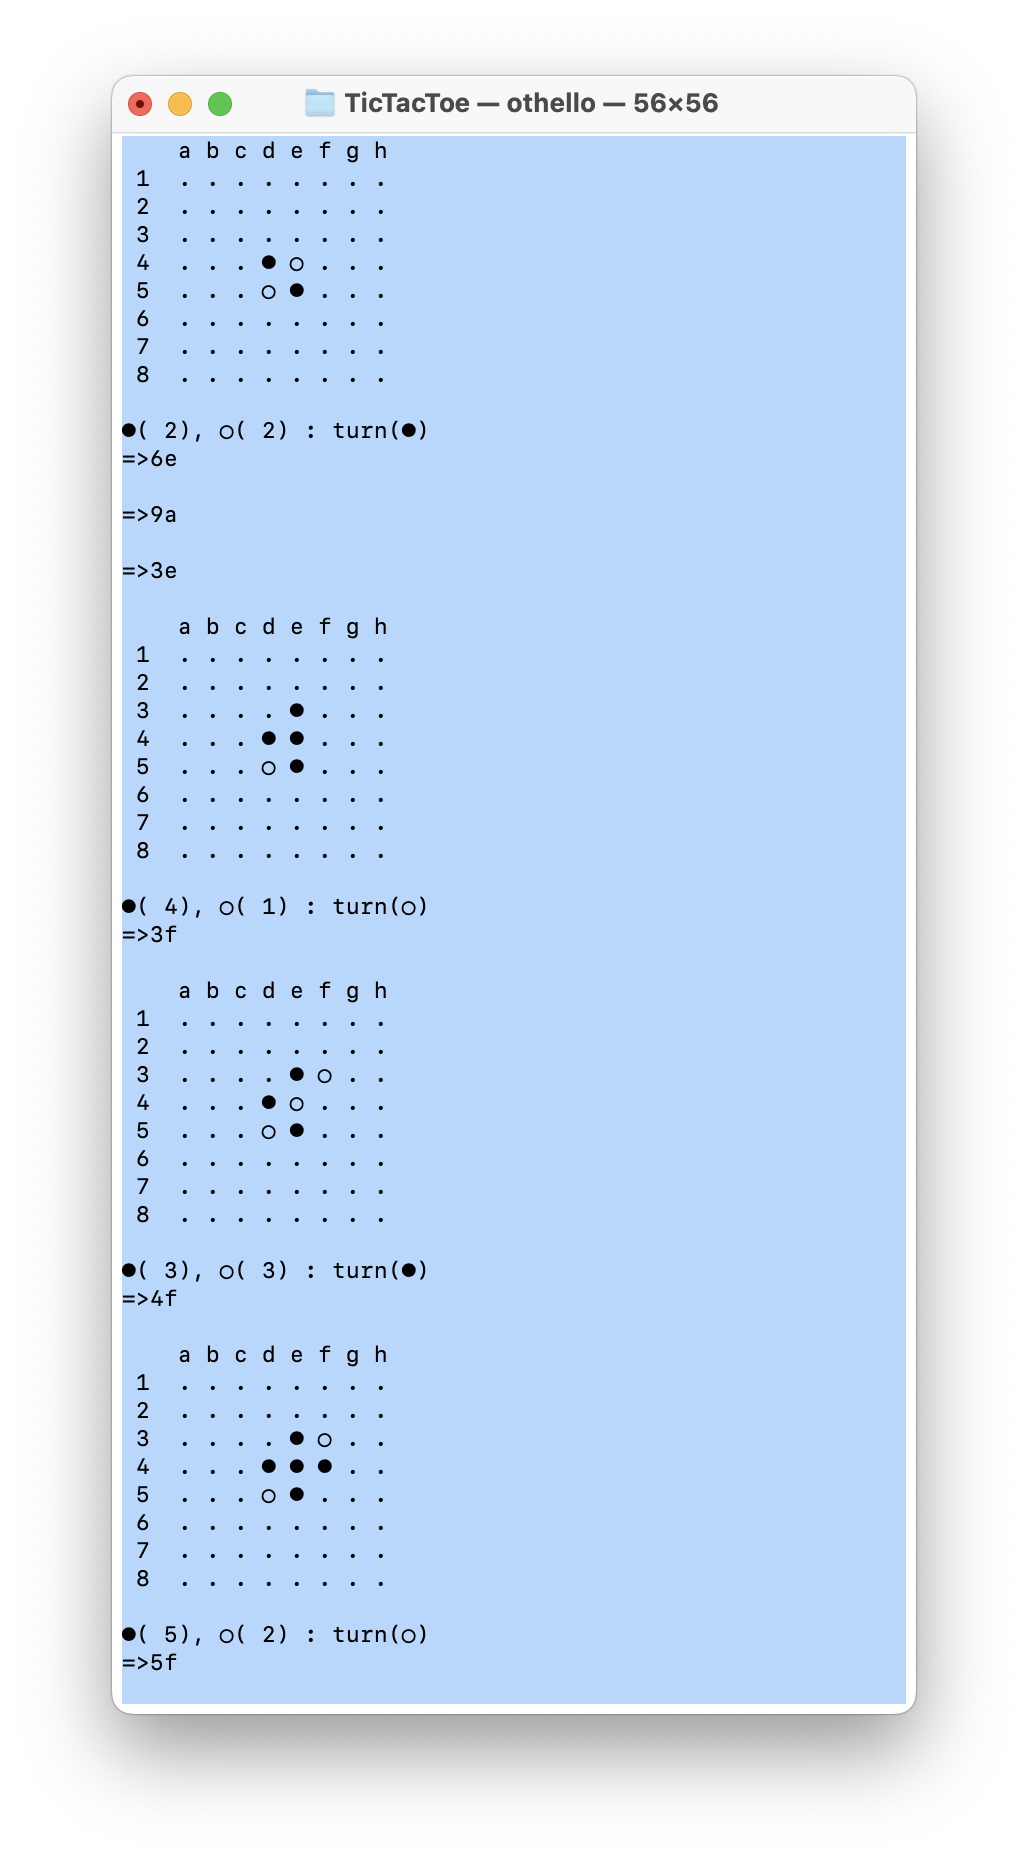
\includegraphics[keepaspectratio,scale=0.5]{othelloview.png}

\newpage

\section{各種宣言など}

\begin{enumerate}
	\item これは冒頭に記述する
	\item BOOLEAN型を enum で定義する
	\item 盤面の幅BOARDWは \#define 文で指定する
	%それは$4 \times 4, 6 \times 6, 8 \times 8$など、4以上8以下の偶数でなければならない
	\item 盤面に黒の石が置かれている場所にはBLACK 、白の石が置かれている場所はWHITE、何も置かれていない場所はNONEで区別する
	\item 現在注目している石の位置(x,y)から見て、下の方向には(0,-1)、右下には(1,-1)、右には(0,1)、右上には(1,1)、上には(1,0)、左上には(-1,1)、左には(-1,0)、左下には(-1,-1)を加えることで、上下、左右、斜め右上下、斜め左上下の、全部で8つの方向の場所を確認していくことができる
	\item 盤面上の場所(x,y)を指定するための構造体POSを定義する
	\item 盤面状態を保持している1次元配列board上の位置は、POS型変数(x,y)から\\$y \times BOARDW +x$によって求める
	\item 手番は変数turnに保持している
	\item パスの回数passcountが2回になるとゲームは終了する
	\item 終了フラグendflagが偽である間ゲームは続く
	\item setstone()関数は盤面の指定位置に石を置く操作
	\item getstone()関数は盤面の指定位置の状態を知る操作
\end{enumerate}

\begin{lstlisting}
	#include <stdio.h>
	#include <stdlib.h>
	
	enum BOOLEAN{
		false,    /* false=0, true=1 */
		true
	};
	
	#define BOARDW (8) // 4, 6, 8, ....
	#define BLACK (0)
	#define WHITE (1)
	#define NONE (2)
	
	int UNITV[][2] = {{0,-1},{1,-1},{1,0},{1,1},{0,1},{-1,1},{-1,0},{-1,-1}};
	int turn = BLACK;
	int passcount = 0;
	int endflag = false;
	int board[BOARDW * BOARDW];
	
	const char* TILE[] = {
		"●",  //TILE_BLACK
		"◯",  //TILE_WHITE
		"."   //TILE_NONE
	};
	
	typedef struct {
		int x, y;
	}POS;
	
	void setstone(POS pos, int num){
		int index = (pos.y * BOARDW) + pos.x;
		board[index] = num;
	}
	
	int getstone(POS pos){
		int index = (pos.y * BOARDW) + pos.x;
		return board[index];
	}
\end{lstlisting}


\section{主処理}

\begin{enumerate}
	\item 行番号(1,2,3,...)と列記号文字(a,b,c,...)の連続する半角2文字で石の位置を指定する
	\item decode()関数を使って、入力された位置の文字列をPOS型変数に変換する(ここに2桁の行番号は想定していない)
	\item 手番の石を置けない場所(盤面の外:!isinside()、又は反転できる石がない:flippable()がゼロ)を指定しても無視する
	\item 現在位置posの周辺8方向に、それぞれsearch()で反転できる石の数を数えて反転していく
\end{enumerate}

\begin{lstlisting}
	POS decode(char* str){
		POS pos;
		pos.x = atoi(str) - 1;
		pos.y = *(str+1) - 'a';
		return pos;
	}
	
	void event(POS pos){
		if(endflag){
			initboard();
			return;
		}
		if(0<passcount){
			nextturn();
			drawboard();
			return;
		}
		if(!isinside(pos))
		return;
		if(0==flippable(pos, turn))
		return;
		for(int i=0; i<8; i++){
			int loop = search(pos, i, turn);
			POS temp = pos;
			for(int j=0; j<loop; j++){
				temp = movepos(temp, i);
				setstone(temp, turn);
			}
		}
		setstone(pos, turn);
		nextturn();
		drawboard();
	}
	
	int main(void){
		if(!initboard())
		return 8;
		char inpt[]="   ";
		while(!endflag){
			printf("=>");
			scanf("%s", inpt);
			POS pos = decode(inpt);
			printf("\n");
			event(pos);
		}
		return 0;
	}
\end{lstlisting}

\section{初期化}

\begin{enumerate}
	\item ゲームの盤面の幅は、4以上8以下の偶数である
\end{enumerate}

\begin{lstlisting}
	enum BOOLEAN initboard(){
		if((BOARDW%2)||(BOARDW<4)||(8<BOARDW))
			return false;
		int x, y;
		POS pos;
		for(y=0; y<BOARDW; y++)
			for(x=0; x<BOARDW; x++){
				pos.x = x; pos.y = y;
				setstone(pos, NONE);
			}
		pos.x = pos.y = BOARDW/2-1;
		setstone(pos, BLACK);
		pos.x = BOARDW/2; pos.y = pos.x-1;
		setstone(pos, WHITE);
		pos.y = BOARDW/2; pos.x = pos.y-1;
		setstone(pos, WHITE);
		pos.x = pos.y = BOARDW/2;
		setstone(pos, BLACK);
		turn = BLACK;
		passcount = 0;
		endflag = false;
		drawboard();
		return true;
	}
\end{lstlisting}

\section{盤面の表示}

\begin{enumerate}
	\item 盤面を表示するたびに、count()関数で石の数を数えて表示している。
\end{enumerate}

\begin{lstlisting}
	int count(int color){
		int num=0;
		for(int i=0; i<(BOARDW * BOARDW); i++)
		if(board[i]==color)
		num++;
		return num;
	}
	
	void drawboard(){
		for(int x=0; x<BOARDW; x++){
			if(x==0){
				printf("    ");
				char a='a';
				for(int i=0; i<BOARDW; i++)
				printf("%c ", a+i);
				printf("\n");
			}
			printf("%2d  ", x+1);
			for(int y=0; y<BOARDW; y++){
				int index = y * BOARDW + x;
				switch(board[index]){
					case BLACK:printf("%s ", TILE[BLACK]);break;
					case WHITE:printf("%s ", TILE[WHITE]);break;
					case NONE: printf("%s ", TILE[NONE]); break;
				}
			}
			printf("\n");
		}
		printf("\n%s(%2d), %s(%2d)",TILE[BLACK],count(BLACK),TILE[WHITE],count(WHITE));
		if(!endflag)
		printf(" : turn(%s)\n", TILE[turn]);
		else
		printf("\n");
	}
\end{lstlisting}

\section{手番の交代}

\begin{enumerate}
	\item isinside()関数は、指定された場所が盤の内部の位置かどうかを調べる
	\item flippable()関数は、相手の石を何枚反転させられるかを調べる
	\item movepos()関数は、着目点を現在位置posから上下左右斜めの8方向に移動させる
	\item search()関数は、vで指示された方向に何個の石を反転させられるかを数えている
	\item nextturn()関数では、\\石を置ける空いてる場所があるかどうかを調べて無かったら終了フラグを立てる\\
	指定位置posが相手の石を反転できる場所ならパスの回数をリセットする\\
	パスの回数が2回続いたら終了フラグを立てる
\end{enumerate}

\begin{lstlisting}
	POS movepos(POS pos, int v){
		POS p;
		p.x = pos.x + UNITV[v][0];
		p.y = pos.y + UNITV[v][1];
		return p;
	}
	
	enum BOOLEAN isinside(POS pos){
		if( (pos.x<0) || (BOARDW<=pos.x) )
		return false;
		if( (pos.y<0) || (BOARDW<=pos.y) )
		return false;
		return true;
	}
	
	int search(POS pos, int v, int num){
		int piece = 0;
		while(true){
			pos = movepos(pos, v);
			if(!isinside(pos))
			return 0;
			if(getstone(pos)==NONE)
			return 0;
			if(getstone(pos)==num)
			break;
			piece ++;
		}
		return piece;
	}
	
	int flippable(POS pos, int num){
		if(getstone(pos)!=NONE)
		return 0;
		int total = 0;
		int vec[]={0,0};
		for(int i=0; i<8; i++)
		total += search(pos, i, num);
		return total;
	}
	
	void nextturn(){
		turn ^= 1;
		int empty = 0;
		for(int y=0; y<BOARDW; y++)
		for(int x=0; x<BOARDW; x++){
			POS pos; pos.x=x; pos.y=y;
			if(getstone(pos)==NONE)
			empty++;
			if(0<flippable(pos,turn)){
				passcount = 0;
				return;
			}
		}
		if(empty==0){
			endflag = true;
			return;
		}
		passcount++;
		if(2<=passcount)
		endflag = true;
	}
\end{lstlisting}

\appendix

\chapter{全体プログラム}

\section{三目並べ}

\lstinputlisting[caption=Tic Tac Toe(三目並べ),label=tictactoe]{../src/tictactoe.c}

\newpage

\section{スライド・パズル}

\lstinputlisting[caption=スライド・パズル,label=slidetile]{../src/slidetile.c}

\newpage

\section{神経衰弱}

\lstinputlisting[caption=神経衰弱,label=flipcard]{../src/flipcard.c}

\newpage

\section{オセロ(リバーシ)}

\lstinputlisting[caption=オセロ,label=othello]{../src/othello.c}

%%%%\chapter{おわりに}
%
%%%%\section*{謝辞}
%%%%\addcontentsline{toc}{chapter}{謝辞}
%

%
\begin{thebibliography}{99}
	\bibitem{1} 田中賢一郎、「ゲームで学ぶ Java Script 入門」、インプレス
	\bibitem{2} 松原拓也(有限会社ニコ)、「Pythonでリバーシを作ろう」、日経ソフトウェア2023年5月号
\end{thebibliography}
%
% END DOCUMENT
\end{document}
%